\documentclass[border=3mm]{article}

\usepackage{pgfplots}

% Unit circle plot style
\pgfplotsset{unit circle/.style={width=4cm,height=4cm,axis lines=middle,xtick=\empty,ytick=\empty,axis equal,enlargelimits,xmax=1.4,ymax=1.4,xmin=-1.4,ymin=-1.4,domain=0:pi/2}}

\begin{document}
	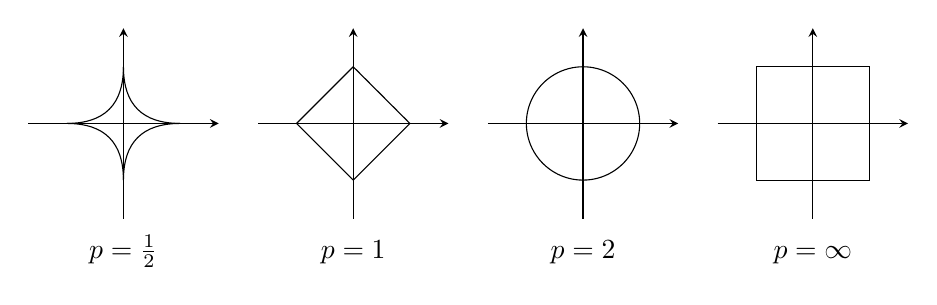
\begin{tikzpicture}
		\coordinate (prev); % Store previous plot position
		\foreach \p / \t in {4/\frac{1}{2}, 2/1, 1/2, 0.0001/\infty} { % Loop through the plots to draw
			% \p is the exponent in the function to plot
			% \t is the p parameter to print
			\begin{axis}[at={(prev)},unit circle,anchor=west]
				\foreach \ss in {1,-1} {
					\foreach \cs in {1,-1} {
						\addplot[] ({\cs*(cos(deg(x)))^\p},{\ss*(sin(deg(x))^\p});
					}
				}
			\end{axis}
			\node[below=0.5cm, anchor=base] at (current axis.south) {$p=\t$}; % Print p
			\coordinate[right=0.5cm] (prev) at (current axis.east) ; % Set position for next plot
		}
	\end{tikzpicture}
	
	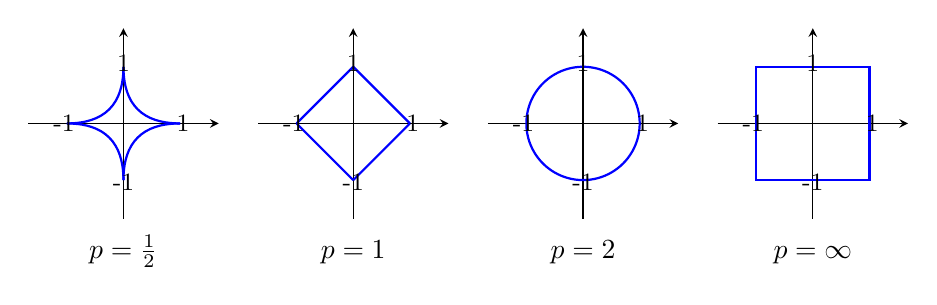
\begin{tikzpicture}
		\coordinate (prev); % Store previous plot position
		\foreach \p / \t in {4/\frac{1}{2}, 2/1, 1/2, 0.0001/\infty} { % Loop through plots
			\begin{axis}[at={(prev)},unit circle,anchor=west]
				% Draw unit circle (dashed gray)
				%\addplot [gray, dashed, domain=0:360, samples=200] ({cos(x)}, {sin(x)});
				
				% Plot the normed shape
				\foreach \ss in {1,-1} {
					\foreach \cs in {1,-1} {
						\addplot [blue, thick] 
						({\cs*(cos(deg(x)))^\p},{\ss*(sin(deg(x)))^\p});
					}
				}
				
				% Add +1 and -1 labels
				\node[font=\small] at (axis cs:1.05,0) {1};
				\node[font=\small] at (axis cs:-1.05,0) {-1};
				\node[font=\small] at (axis cs:0,1.05) {1};
				\node[font=\small] at (axis cs:0,-1.05) {-1};
			\end{axis}
			\node[below=0.5cm, anchor=base] at (current axis.south) {$p=\t$}; % Label under plot
			\coordinate[right=0.5cm] (prev) at (current axis.east); % Move to next position
		}
	\end{tikzpicture}
	
	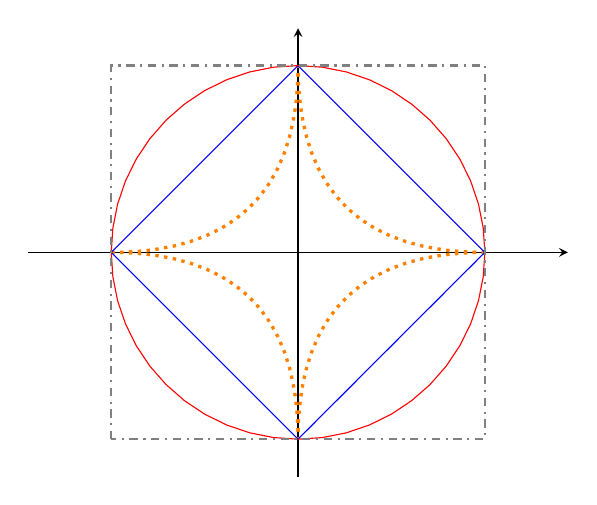
\begin{tikzpicture}
		\begin{axis}[axis lines=middle,xtick=\empty,ytick=\empty,axis equal,enlargelimits,xmax=1,ymax=1,xmin=-1,ymin=-1]
			%p=0.5
			\begin{scope}[very thick,dotted,orange,domain=0:pi,samples=50]
				\addplot[] ({(cos(deg(x)))^(4},{ (sin(deg(x))^(4});
				\addplot[] ({(cos(deg(x)))^(4},{ -(sin(deg(x))^(4});
				\addplot[] ({-(cos(deg(x)))^(4},{ (sin(deg(x))^(4});
				\addplot[] ({-(cos(deg(x)))^(4},{-(sin(deg(x))^(4});
			\end{scope}
			%p=1
			\addplot[blue,domain=0:pi] ({(cos(deg(x)))^2},{(sin(deg(x))^2});
			\addplot[blue,domain=0:pi] ({(cos(deg(x)))^2},{-(sin(deg(x))^2});
			\addplot[blue,domain=0:pi] ({-(cos(deg(x)))^2},{(sin(deg(x))^2});
			\addplot[blue,domain=0:pi] ({-(cos(deg(x)))^2},{-(sin(deg(x))^2});
			%p=2
			\addplot[red,domain=-pi:0] ({(cos(deg(x)))},{(sin(deg(x))});
			\addplot[red,domain=0:pi] ({(cos(deg(x)))},{(sin(deg(x))});
			%p=inf
			\draw[thick,dashdotted,gray] (axis cs:-1,-1) rectangle (axis cs:1,1);
		\end{axis}
	\end{tikzpicture}
	
	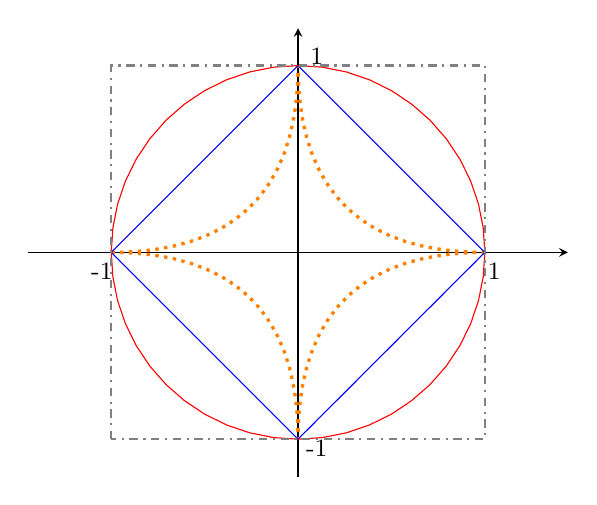
\begin{tikzpicture}
		\begin{axis}[axis lines=middle,xtick=\empty,ytick=\empty,axis equal,enlargelimits,xmax=1,ymax=1,xmin=-1,ymin=-1]
			%p=0.5
			\begin{scope}[very thick,dotted,orange,domain=0:pi,samples=50]
				\addplot[] ({(cos(deg(x)))^(4},{ (sin(deg(x))^(4});
				\addplot[] ({(cos(deg(x)))^(4},{ -(sin(deg(x))^(4});
				\addplot[] ({-(cos(deg(x)))^(4},{ (sin(deg(x))^(4});
				\addplot[] ({-(cos(deg(x)))^(4},{-(sin(deg(x))^(4});
			\end{scope}
			%p=1
			\addplot[blue,domain=0:pi] ({(cos(deg(x)))^2},{(sin(deg(x))^2});
			\addplot[blue,domain=0:pi] ({(cos(deg(x)))^2},{-(sin(deg(x))^2});
			\addplot[blue,domain=0:pi] ({-(cos(deg(x)))^2},{(sin(deg(x))^2});
			\addplot[blue,domain=0:pi] ({-(cos(deg(x)))^2},{-(sin(deg(x))^2});
			%p=2
			\addplot[red,domain=-pi:0] ({(cos(deg(x)))},{(sin(deg(x))});
			\addplot[red,domain=0:pi] ({(cos(deg(x)))},{(sin(deg(x))});
			%p=inf
			\draw[thick,dashdotted,gray] (axis cs:-1,-1) rectangle (axis cs:1,1);
		
			% Add +1 and -1 labels
			\node[font=\small] at (axis cs:1.05,-0.1) {1};
			\node[font=\small] at (axis cs:-1.05,-0.1) {-1};
			\node[font=\small] at (axis cs:0.1,1.05) {1};
			\node[font=\small] at (axis cs:0.1,-1.05) {-1};		
		
		\end{axis}
	\end{tikzpicture}
	    
	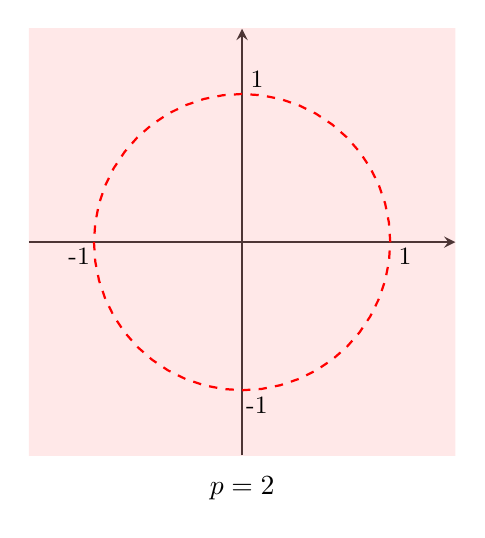
\begin{tikzpicture}
		\begin{axis}[
			width=7cm, height=7cm,
			axis lines=middle,
			xtick=\empty, ytick=\empty,
			axis equal,
			enlargelimits,
			xmin=-1.2, xmax=1.2,
			ymin=-1.2, ymax=1.2,
			thick,
			domain=0:90
			]
			
			\draw [fill = red!30, opacity=0.3, draw=none]  (axis cs:0,0) circle[radius=100];
			
			%p=2
			\addplot[red,domain=-pi:0,  thick, dashed] ({(cos(deg(x)))},{(sin(deg(x))});
			\addplot[red,domain=0:pi,  thick, dashed] ({(cos(deg(x)))},{(sin(deg(x))});
			
			
			% Add +1 and -1 labels
			\node[font=\small] at (axis cs:1.1,-0.1) {1};
			\node[font=\small] at (axis cs:-1.1,-0.1) {-1};
			\node[font=\small] at (axis cs:0.1,1.1) {1};
			\node[font=\small] at (axis cs:0.1,-1.1) {-1};		
			
		\end{axis}
		\node[below=0.5cm, anchor=base] at (current axis.south) {$p=2$}; % Print p
	\end{tikzpicture}
 
 
	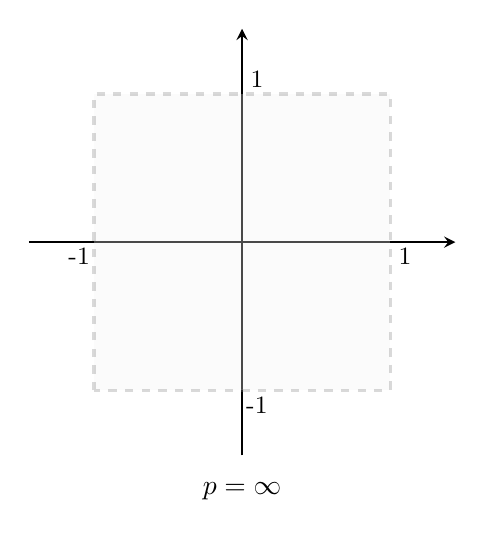
\begin{tikzpicture}
		\begin{axis}[
			width=7cm, height=7cm,
			axis lines=middle,
			xtick=\empty, ytick=\empty,
			axis equal,
			enlargelimits,
			xmin=-1.2, xmax=1.2,
			ymin=-1.2, ymax=1.2,
			thick,
			domain=0:90
			]
			
			%p=inf
			\draw[very thick, dashed, gray, fill=gray!10, opacity=0.3,] (axis cs:-1,-1) rectangle (axis cs:1,1);
			
			% Add +1 and -1 labels
			\node[font=\small] at (axis cs:1.1,-0.1) {1};
			\node[font=\small] at (axis cs:-1.1,-0.1) {-1};
			\node[font=\small] at (axis cs:0.1,1.1) {1};
			\node[font=\small] at (axis cs:0.1,-1.1) {-1};		
			
		\end{axis}
		\node[below=0.5cm, anchor=base] at (current axis.south) {$p=\infty$}; % Print p
	\end{tikzpicture}
  
	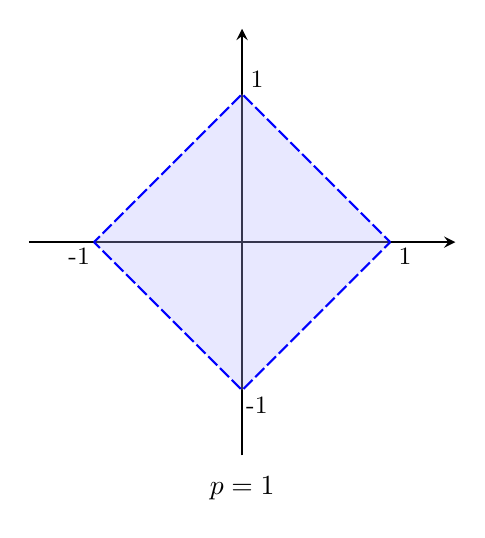
\begin{tikzpicture}
		\begin{axis}[
			width=7cm, height=7cm,
			axis lines=middle,
			xtick=\empty, ytick=\empty,
			axis equal,
			enlargelimits,
			xmin=-1.2, xmax=1.2,
			ymin=-1.2, ymax=1.2,
			thick,
			domain=0:90
			]
			
			\addplot  [fill=blue!30, opacity=0.3, draw=none] coordinates { (0,1) (-1,0) (0,-1) (1,0)}
			--cycle;
			
			
			\foreach \sx in {1,-1} {
				\foreach \sy in {1,-1} {
					\addplot[blue, domain=0:pi,  thick, dashed]
					({\sx*(cos(deg(x)))^2}, {\sy*(sin(deg(x)))^2});
				}
			}
			
			% Add +1 and -1 labels
			\node[font=\small] at (axis cs:1.1,-0.1) {1};
			\node[font=\small] at (axis cs:-1.1,-0.1) {-1};
			\node[font=\small] at (axis cs:0.1,1.1) {1};
			\node[font=\small] at (axis cs:0.1,-1.1) {-1};		
			
		\end{axis}
		\node[below=0.5cm, anchor=base] at (current axis.south) {$p=1$}; % Print p
	\end{tikzpicture}
 

	
\end{document}